\documentclass[11pt]{article}

% Use Helvetica font.
%\usepackage{helvet}

%\usepackage[T1]{fontenc}
%\usepackage[sc]{mathpazo}
\usepackage{color}
\usepackage{amsmath,amsthm,amssymb,multirow,paralist}
\usepackage{graphicx} 
%\renewcommand{\familydefault}{\sfdefault}

% Use 1/2-inch margins.
\usepackage[margin=0.8in]{geometry}
\usepackage{hyperref}

\begin{document}

\begin{center}
{\Large \textbf{COM S 474/574: Introduction to Machine Learning}

Homework \#2}\\
\vspace{0.2cm}
\textbf{Name:} Miles Nichols\\

\linethickness{1mm}\line(1,0){498}

\begin{enumerate}
\item Please put required code files or report into a
compressed file ``HW\#\_FirstName\_LastName.zip''
\item Unlimited number of submissions are
allowed on Canvas and the latest one will be graded.
\item {\color{red} No later submission is accepted.}
\item Please read and follow submission instructions. No exception
will be made to accommodate incorrectly submitted files/reports.
\item All students are required to typeset their reports using
latex. Overleaf
(\url{https://www.overleaf.com/learn/latex/Tutorials}) can be a
good start.
\end{enumerate}

\linethickness{1mm}\line(1,0){498}

\end{center}

%%%%%%%%%%%%%%%%%%%%%%%%%%%%%%%%%%%%%%%%%%%%%%%%%%%%%%%%%%%%%%%%%%%%%%%%%%%%%%%

%%%%%%%%%%%%%%%%%%%%%%%%%%%%%%%%%%%%%%%%%%%%%%%%%%%%%%%%%%%%%%%%%%%%%%%%%%%%%%%

\begin{enumerate}

\item (60 points) \textbf{Perceptron for Handwritten Digits Recognition}:
The handwritten digits files are in the ``data'' folder: train.txt
and test.txt. The starting code is in the ``code'' folder. In the
data file, each row is a data example. The first entry is the digit
label (``1'' or ``5''), and the next 256 are grayscale values
between -1 and 1. The 256 pixels correspond to a $16\times16$ image.
You are expected to implement your solution based on the given
codes. The only file you need to modify is the ``solution.py'' file.
You can test your solution by running ``main.py" file. Note that
code is provided to compute a two-dimensional feature (symmetry and
average intensity) from each digit image; that is, each digit image
is represented by a two-dimensional vector before being augmented
with a ``1'' to form a three-dimensional vector as discussed in
class. These features along with the corresponding labels should
serve as inputs to your Perceptron algorithm.
{\color{red}You are expected to use Python3.}

\begin{enumerate}
\item (10 points) Familiarize yourself with the data by completing the \emph{show\_images} function. Include the images you plotted in your report.

\begin{center}
    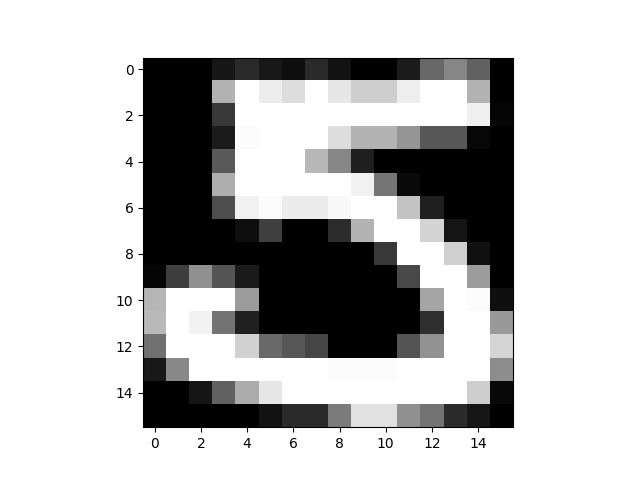
\includegraphics[width=0.6\textwidth]{image_1.png}
\end{center}
\begin{center}
    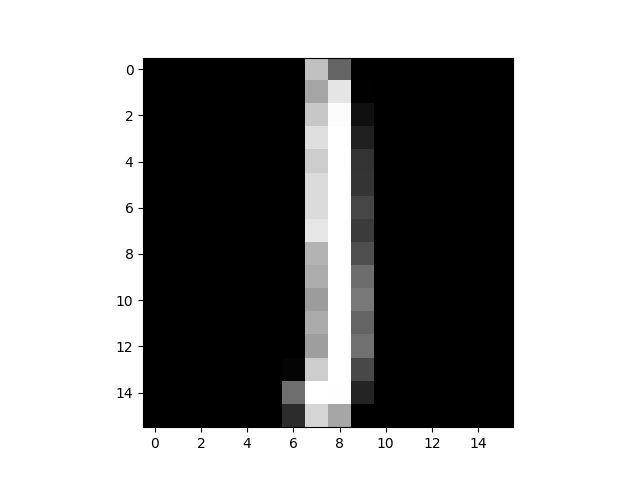
\includegraphics[width=0.6\textwidth]{image_2.png}
\end{center}


\item (10 points) In this assignment, we have already extracted two features, symmetry and
average intensity, to distinguish between 1 and 5. Familiarize
yourself with the features by completing the \emph{show\_features}
function and include the 2-D scatter plot into your report. For each
sample, plot the two features with a red \textcolor{red}{$*$} if the
label is 1 and a blue \textcolor{blue}{$+$} if the label is 5.

\begin{center}
    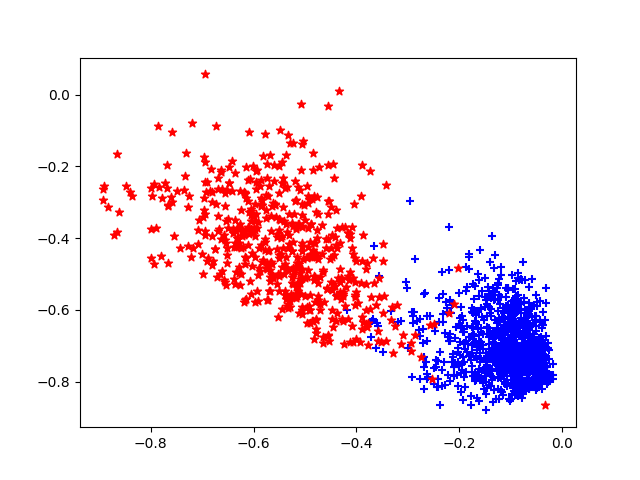
\includegraphics[width=0.7\textwidth]{train_features.png}
\end{center}

\item (20 points) Complete the \emph{Perceptron} class. You can test your
accuracy results using the ``test\_accuracy'' function in
``main.py''.

\textbf{Accuracy Results:}
After completing the Perceptron class  and testing the model across different maximum iterations, the algorithm yielded the following results:
\begin{itemize}
    \item \textbf{Max Iteration 10:} Train Accuracy: 0.981422, Test Accuracy: 0.959906
    \item \textbf{Max Iteration 30:} Train Accuracy: 0.976938, Test Accuracy: 0.948113
    \item \textbf{Max Iteration 50:} Train Accuracy: 0.976938, Test Accuracy: 0.948113
    \item \textbf{Max Iteration 100:} Train Accuracy: 0.976297, Test Accuracy: 0.948113
    \item \textbf{Max Iteration 200:} Train Accuracy: 0.976297, Test Accuracy: 0.948113
\end{itemize}

\item (20 points) Complete the \emph{show\_result} function to plot the
test data with the separators. Include the images you plotted into
your report.

\begin{center}
    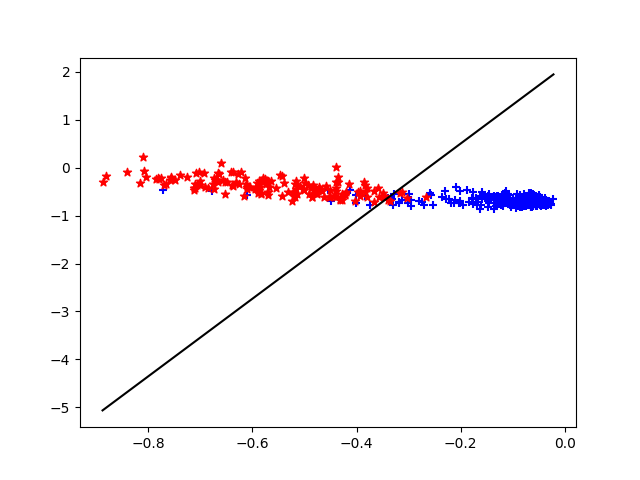
\includegraphics[width=0.7\textwidth]{result.png}
\end{center}

\textbf{Analysis:}
The Perceptron model successfully learns to separate the handwritten ``1''s (red stars) from the ``5''s (blue crosses). However, because there is slight overlap between the two classes near the center of the distribution, the data is not perfectly linearly separable. This is why the model performs best at 10 iterations with the highest accuracy. With more iterations, the model continues adjusting back and forth to try and accommodate for each misclassified data point. This ultimately ends up giving diminishing the accuracy. 

\end{enumerate}

\end{enumerate}

\end{document}